% =========================================================================== %
% Yes. This is a document.

\documentclass[
	english,
	aspectratio=169,
	table
]{beamer}

% =========================================================================== %
% Theme
\usepackage{scrlfile}
	\ReplacePackage{beamerthemeSHUR}{./sty/beamerthemeSHUR}
	\ReplacePackage{beamerinnerthemefancy}{./sty/beamerinnerthemefancy}
	\ReplacePackage{beamerouterthemedecolines}{./sty/beamerouterthemedecolines}
	\ReplacePackage{beamercolorthemechameleon}{./sty/beamercolorthemechameleon}

\usetheme[
	pageofpages=/,
	bullet=circle,
	titleline=true,
	alternativetitlepage=true,
	watermark="",
	watermarkheight=0px,
	watermarkheightmult=0
	]
{SHUR}

% =========================================================================== %
% the usual stuff

\usepackage[utf8]{inputenc}
\usepackage[T1]{fontenc}
\usepackage{babel}
\usepackage{lmodern}
\usepackage{microtype}
\usepackage{csquotes}
\usepackage{xspace}
\usepackage{ulem}

\usepackage{tabularx}
\usepackage{booktabs}
\usepackage{multirow}

\usepackage{color, colortbl}
\usepackage{xcolor}
	\definecolor{tabhighlight}{RGB}{230,240,255}

\usepackage{tabto}
\usepackage{setspace}

\usepackage{minted}
	\usemintedstyle{friendly}

\usepackage{tikz}
	\usetikzlibrary{positioning}
	\usetikzlibrary{matrix}
	\usetikzlibrary{shapes.geometric}
	\usetikzlibrary{backgrounds}
	\usetikzlibrary{calc}
	\usetikzlibrary{decorations.pathreplacing}
	\tikzstyle{every picture}+=[remember picture] 
\usepackage{adjustbox}

\usepackage{amsmath}
\usepackage{physics}

\usepackage[most]{tcolorbox}
	\tcbsetforeverylayer
		{colback=cyan!10!white,
		 colframe=cyan!75!black,
		 arc=0pt,
		 outer arc=0pt
		}
	\newtcolorbox{codebox}[1][Code]
		{colback=black!5!white,
		 colframe=blue!40!black,
		 title=#1,
		 leftupper=6mm
		}
	\newtcolorbox{cmdbox}[1][Command Line]
		{colback=black,
		 coltext=white,
		 fontupper=\ttfamily ,
		 colframe=blue!40!black,
		 title=#1,
		 outer arc=0pt
		}
	\newtcolorbox{warnbox}[1][Warning]
		{colback=black!5!white,
		 colframe=red!40!black,
		 title=#1
		}
	\newtcolorbox{hintbox}[1][Hint]
		{colback=black!5!white,
		 colframe=green!40!black,
		 title=#1
		}
	\newtcolorbox{defbox}[1][Code]
		{colback=cyan!10!white,
		 colframe=cyan!90!black,
		 title=#1
		}
	\newtcolorbox{recapbox}[1][Code]
		{colback=yellow!10!white,
		 colframe=yellow!90!black,
		 coltitle=black,
		 title=#1
		}
%==============================================================================%
% GLOBAL MACROS

\newcommand*{\zB}{e.\,g. }
\newcommand*{\ie}{i.\,e. }

\newcommand{\Thus}{\ensuremath{\Rightarrow}\xspace}
\newcommand{\thus}{\ensuremath{\rightarrow}\xspace}

\newcommand*{\tabcrlf}{\\ \midrule}			% actually still allows for optional argument

\newcommand*{\inPy}[1]{\mintinline{python}{#1}}

\newcommand*{\todo}[1]{{\color{red}TODO: #1}}
\newcommand*{\sfrac}[2]{\ensuremath{{}^{#1}/_{#2}}}

% =========================================================================== %

\author{Stefan Hartinger}
\title{Python for Scientists}
\subtitle{Part 22: Markup Languages: HTML and XML}
\institute{Department of Just Some Dude Who Likes to Talk}
\date{Winter 2023/24}

% =========================================================================== %

\begin{document}
\normalem   % package ulem (used for strikethrough formatting) redefines \emph to mean underline. This restores the default
\newcommand{\rx}[1]{\texttt{"{\color{olive}#1}"}}
\newcommand{\match}[1]{{\color{blue}#1}}
\newcommand{\qtt}[1]{\texttt{"{#1}"}}

% =========================================================================== %

\begin{frame}[t,plain]
\titlepage
\end{frame}

% =========================================================================== %

\begin{frame}[fragile]{Tags}
%
\begin{center}

\includegraphics[width=.9\linewidth]{./gfx/22-xkcd-tags}

\emph{\phantom{.}<A>: Like</a>this.\&nbsp;}

\vspace{6pt}
Source: \url{https://xkcd.com/1144/}
\end{center}
%
\end{frame}

% =========================================================================== %

\begin{frame}{Scope For Today}
%
\begin{itemize}
\item Markup Languages in General
	\begin{itemize}
	\item Attack of the Acronyms: HTML, XML, XHTML, SGML, DTD, XSD
	\item Tag structure
	\end{itemize}
\item Intro to HTML
	\begin{itemize}
	\item Some important tags to know
	\item Semantic vs. structural tags
	\item The HTML \texttt{head} block
	\end{itemize}
\item Fantastic XMLs and where to find them
	\begin{itemize}
	\item Settings Files of PyCharm
	\item Open Document Format
	\end{itemize}
\item Bringing Python into the mix: 
	\begin{itemize}
	\item \texttt{html.parser}
	\item \texttt{xml.etree.ElementTree}
	\end{itemize}
\end{itemize}
%
\end{frame}

% =========================================================================== %

\begin{frame}{What is a MarkUp?}
%
\begin{columns}[T]
\column{.5\linewidth}
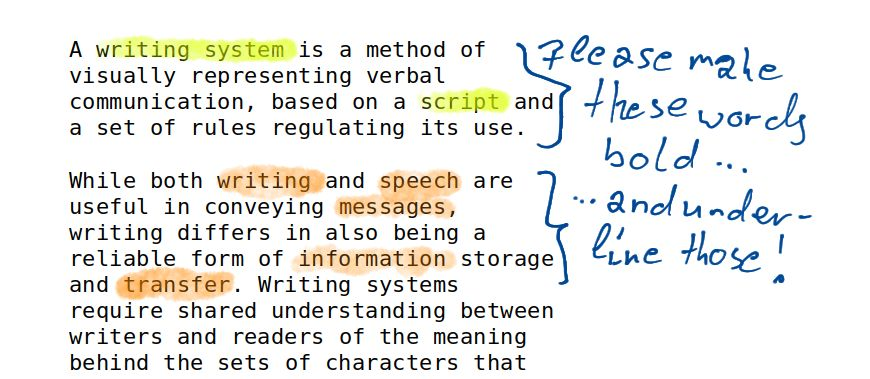
\includegraphics[width=\linewidth]{./gfx/22-markup}

\begin{itemize}
\item These are markups
\item Historically, a typographer would add handwritten notes for the printer to manuscripts
	\begin{itemize}
	\item E.\;g. type face, size, style
	\end{itemize}
\end{itemize}
%
\pause
%
\column{.5\linewidth}
\begin{itemize}
\item In computing: basically same concept
\item Adding metainformation to text
	\begin{itemize}
	\item Formatting
	\item Other semantics, \zB \emph{this is a hyperlink}
	\end{itemize}
\pause
\item Implies a syntax to distinguish text from markups
	\begin{itemize}
	\item How to express metainformation
	\item How to transcribe text that looks like metainformation
	\end{itemize}
\pause
\item Multitude of markup languages published
	\begin{itemize}
	\item \LaTeX
	\item Markdown
	\item XML, HTML
	\end{itemize}
\end{itemize}
\end{columns}
%
\end{frame}

% =========================================================================== %

\begin{frame}{Attack of the Acronyms}
%
\begin{description}
\item[SGML] \emph{Standard Generalized Markup Language} -- meta language that defines how markups look like and how to distinguish markups from text
\pause
\item[HTML] \emph{Hypertext Markup Language} -- an instance of SGML, used to describe websites
\pause
\item[DTD]  \emph{Document Type Definition} -- fixes the rules for an instance of an SGML
	\begin{itemize}
	\item Example: \url{https://www.w3.org/TR/html401/sgml/dtd}
	\item Defines \emph{HTML 4.01}
	\end{itemize}
\pause
\item[XML]  \emph{Extensible Markup Language} -- stricter variant of SGML, better machine readable
	\begin{itemize}
	\item There are also instantiations of XML for specific contexts
	\item[\Thus] We have to distinguish between the meta-language XML and concrete realizations for a given context
	\end{itemize}
\pause
\item[XSD]  \emph{XML Schema Definition} -- alternative to DTDs sometimes used with XML
\pause
\item[XHTML] The XML-compliant version of HTML
\end{description}
%
\end{frame}

% =========================================================================== %

\begin{frame}{Structure of XML-Like Documents (1)}
%
\begin{itemize}
\item Primary element: \emph{Tag}
	\begin{itemize}
	\item A \texttt{keyword} in <angular brackets>
		\begin{itemize}
		\item \texttt{keyword} must not contain whitespaces, tabs, ...
		\item Context defines, which keywords are allowed
		\end{itemize}
	\end{itemize}
\pause
\item Tag may contain text
	\begin{itemize}
	\item Distinguish between \emph{opening tags} (\texttt{<keyword>}) and \emph{closing tags} (\texttt{<{\color{red}/}keyword>})
	\item Text between an opening and closing tag is the contained text
	\item Example:\\
		\texttt{not tagged <tag>tagged text</tag> again not tagged}
	\item Empty tags: end with a slash (\texttt{<keyword {\color{red}/}>})
	\item SGML/HTML: tags need not be closed
	\end{itemize}
\pause
\item Tags may contain an arbitrary number of attributes
	\begin{itemize}
	\item Attribute: key-value pairs
	\item \texttt{key="value"} within the opening tag brackets
	\item Single or double quotes; optional but highly recommended
	\item Example:
		\mintinline{xml}{<tag key1="value 1" key2='value 2'>text<tag>}
	\end{itemize}
\end{itemize}
%
\end{frame}

% =========================================================================== %

\begin{frame}{Structure of XML-Like Documents (2)}
%
\begin{itemize}
\item Tags are case sensitive
	\begin{itemize}
	\item \texttt{<tag>}, \texttt{<Tag>} and \texttt{<TAG>} are different objects
	\item By convention, we only use lower case tags
	\end{itemize}
\pause
\item Tags may be nested
	\begin{itemize}
	\item Simply several opening tags in sequence ...
	\item ... followed by text (optional) ...
	\item ... followed by closing text \textbf{in reverse order}
	\item Example:
		\texttt{{\color{blue}<tag\_1>}{\color{red}<tag\_2>}text {\color{green}<tag\_without\_text />} {\color{red}text</tag\_2>}{\color{blue}</tag\_1>}}
	\item \textbf{Only one root element}
	\end{itemize}
\pause
\item Some tags only allowed nested in certain others
	\begin{itemize}
	\item Depends on keyword and context
	\item Example: table alignment tags only make sense when in a table context
	\end{itemize}
\end{itemize}
%
\end{frame}

% =========================================================================== %

\begin{frame}[fragile]{Structure of XML-Like Documents (3)}
%
\begin{itemize}
\item Indentation and linebreaks are ignored
	\begin{itemize}
	\item Single whitespace is meaningful
	\item Multiple whitespaces, tabs, ... are treated like a single whitespace.
	\item Makes the raw markup code better legible
	\item Requires special syntax elements to encode line breaks and whitespaces
	\item Example: these two are syntactically equivalent:
		\begin{itemize}
		\item \mintinline{html}{<ul><li>Tags may be nested</li><li>Indentation ignored</li></ul>}
		\item \begin{minted}{html}
<ul>
  <li>Tags may be nested</li>
  <li>Indentation ignored</li>
</ul>
		\end{minted}
		\end{itemize}
	\end{itemize}
\pause
\item Exceptions
	\begin{itemize}
	\item Attribute values: whitespaces are stored verbatim
	\item XML: whitespaces and linebreaks in contained text preserved
	\end{itemize}
\end{itemize}
%
\end{frame}

% =========================================================================== %

\begin{frame}{Structure of XML-Like Documents (4)}
%
\begin{itemize}
\item Comments
	\begin{itemize}
	\item Begin with \texttt{<!-{}-} and end with \texttt{-{}->}
	\item May be multiline
	\end{itemize}
\pause
\item Special entities
	\begin{itemize}
	\item Text may not contain \texttt{<}, \texttt{>}, \texttt{'}, \texttt{"} or \texttt{\&}
	\item Instead: Escape sequence \texttt{\&code;}, in which \texttt{code} is ...
		\begin{itemize}
		\item either is a decimal code point (like an ASCII-Code, but allows values greater than 127)
		\item or a human-readable token like \texttt{amp} (\texttt{\&}), \texttt{lt} (\texttt{<}), \texttt{gt} (\texttt{>})
		\item See also \url{https://oinam.github.io/entities/}
		\end{itemize}
	\end{itemize}
\pause
\item Prolog: DOCTYPE and XML-Declaration
	\begin{itemize}
	\item XML documents \sout{must} should begin with \mintinline{xml}{<?xml version="1.0" ?>}
		\begin{itemize}
		\item Optionally (and recommended): attributes \texttt{encoding="UTF-8"} and \texttt{standalone="yes"}
		\end{itemize}
	\pause
	\item SGML documents \sout{must} should begin with \texttt{<!DOCTYPE type>} (in XML: second line)
		\begin{itemize}
		\item Type specifies the SGML implementation, \zB \texttt{html}
		\item Optional attributes: \texttt{<!DOCTYPE type PUBLIC uri dtd>}
		\item \texttt{uri}: some token uniquely identifying the rules for the version of \texttt{type}
		\item \texttt{dtd}: link to the DTD
		\end{itemize}
	\end{itemize}
\end{itemize}
%
\end{frame}

% =========================================================================== %

\begin{frame}[fragile]{Entity Definition and Billion Laughs Attack}
%
\begin{itemize}
\item Entity Definition: Normally in DTD, but also allowed in \texttt{DOCTYPE} part of the prolog
	\begin{itemize}
	\item Square brackets enclose DTD code
	\end{itemize}
\pause
\item Entity Definition
	\begin{itemize}
	\item \mintinline{xml}{<!ENTITY name "content">} (or \mintinline{xml}{<!ENTITY name (#PCDATA)>})
	\item \texttt{content} is an arbitrary string (\texttt{\#PCDATA} defines a new tag)
	\item May contain already defined entities like \texttt{\&gt;}
	\end{itemize}
\end{itemize}
%
\pause
%
\begin{warnbox}[Billion Laughs Attack, leftupper=7mm]
\begin{minted}[linenos, fontsize=\scriptsize]{xml}
<?xml version="1.0"?>       <!-- https://en.wikipedia.org/wiki/Billion_laughs_attack -->
<!DOCTYPE lolz [
 <!ELEMENT lolz (#PCDATA)>                        <!-- this makes 'lolz' a valid tag -->
 <!ENTITY lol1 "lol lol lo lol lol lol lol lol lol lol ">
 <!ENTITY lol2 "&lol1;&lol1;&lol1;&lol1;&lol1;&lol1;&lol1;&lol1;&lol1;&lol1;">
 <!-- ... likewise lol3 through lol9 -->
]>
<lolz>&lol9;</lolz>                    <!-- 10^9 lols, taking up gigabytes of memory -->
\end{minted}
\end{warnbox}
%
\end{frame}

% =========================================================================== %

\begin{frame}{Introduction to HTML}
%
\begin{itemize}
\item Root element: \texttt{html} -- everything else must be contained within
	\pause
	\begin{itemize}
	\item Two allowed sub-elements: \texttt{head} and \texttt{body}
		\begin{itemize}
		\item \texttt{head} is optional and contains meta-information
		\item \texttt{body} is mandatory and contains the website text
		\end{itemize}
	\pause
	\item Tags under \texttt{body} can either communicate \emph{format} (\zB this is \textbf{bold}) or \emph{semantics} \zB this is \textbf{important}
		\begin{itemize}
		\item Semantic information can \emph{optionally }be associated with formatting
		\item May be used by computer programs to make sense of the text
		\end{itemize}
	\pause
	\item Tags under \texttt{head} contains things like ...
		\begin{itemize}
		\item Website title and icon \\
			\vspace{3pt}
			
\includegraphics[width=.8\linewidth]{./gfx/22-html-meta}
		\item Style information (\zB make every headline red and underlined)
		\item Search engine optimization (SEO) information (keywords)
		\item Scaling directives (relevant when website should be viewed both, on desktop computers and mobile devices)
		\end{itemize}
	\end{itemize}
\end{itemize}
%
\end{frame}
 

% =========================================================================== %

\begin{frame}{Basic HTML Tags}
%
\begin{itemize}
\item Text directly under \texttt{body} is displayed as is (modulo whitespaces and linebreaks)
\pause
\item Formatting (direct/semantically)
	\begin{itemize}
	\item \texttt{<b>}/\texttt{<strong>} makes text \textbf{bold}
	\item \texttt{<i>/\texttt{<em>}} makes text \emph{italics}
	\item \texttt{<u>} makes text \underline{underlined}
	\item \texttt{<s>} makes text \sout{strike through}
		\begin{itemize}
		\item Use \texttt{<del>} and \texttt{<ins>} to communicate edits
		\end{itemize}
	\end{itemize}
\pause
\item Headlines get the tags \texttt{<h1>} through \texttt{<h6>} 
	\begin{itemize}
	\item Considered semantic tags
	\end{itemize}
\pause
\item Paragraphs and line breaks
	\begin{itemize}
	\item Recommended: wrap each paragraph in a \texttt{<p>} tag
	\item Alternative (frowned upon): manual line breaks with \texttt{<br/>}
	\end{itemize}
\pause
\item Pictures can be embedded with the \texttt{img} tag
	\begin{itemize}
	\item The picture itself is named in the \texttt{src} attribute
	\item Value for attribute \texttt{src} may be an absolute or relative path
	\item[\Thus] \mintinline{html}{<img src="url" />}
	\end{itemize}
\end{itemize}
%
\end{frame}

% =========================================================================== %

\begin{frame}[fragile]
%
\begin{tcbraster}[raster columns=2,
                  raster equal height,
                  nobeforeafter,
                  raster column skip=0.1cm]
\begin{codebox}[A very basic HTML document]
\begin{minted}[linenos, fontsize=\scriptsize]{xml}
<!DOCTYPE html>
<html>
<body>
<h1>The Headline</h1>
Some introductory text

<h2>A Subchapter</h2>
Even though there are line breaks
     and indentations


in the HTML code, all of this will
be displayed as a single line

<p>Use paragraph tags instead
   to encode line breaks</p>
   
Manual line breaks<br/>work, too.
</body>
</html>
\end{minted}
\end{codebox}
%
\begin{defbox}[Output]
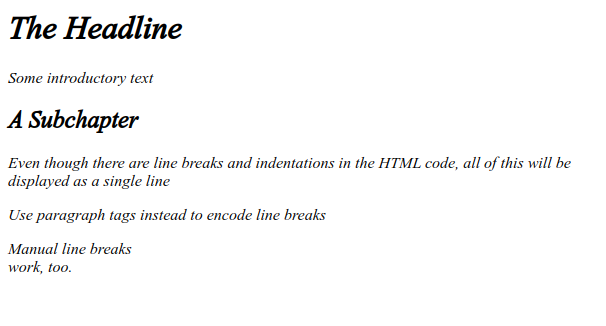
\includegraphics[width=\linewidth]{./gfx/22-html-basic}

\scriptsize
\begin{itemize}
\item Note how subsequent whitespaces are condensed into single spaces
\item Note how linebreaks are ignored
\item Note how \texttt{<p>} adds paragraph spacing while \texttt{<br/>} does not
\item Rendering depends on used browser
\item Browser-independent formatting can be achieved by explicitly stating formats (see later)
\end{itemize}
\end{defbox}
\end{tcbraster}
%
\end{frame}

% =========================================================================== %

\begin{frame}[fragile]{Direct Formatting: \texttt{style} and \texttt{class}}
%
\begin{itemize}
\item Global HTML attributes (can be used with any tag): \texttt{style} and \texttt{class}
	\begin{itemize}
	\item Both used to assign concrete formatting information to the tag
	\item \texttt{style="styledef;"}: use explicit style definition \texttt{styledef}
		\begin{itemize}
		\item \texttt{styledef} are concrete instructions like setting font size, colour, ...
		\end{itemize}
	\item \texttt{class="classid"}: use previously defined format with id \texttt{classid}
		\begin{itemize}
		\item The definitions behind \texttt{classid} are encoded in the \texttt{head} -- see later
		\item Briefly: definitions behind \texttt{classid} are the same as behind a \texttt{styledef}
		\item \texttt{styledef} overrides \texttt{classid}
		\end{itemize}
	\end{itemize}
\pause
\item \texttt{styledef}, aka CSS properties
	\begin{itemize}
	\item Semicolon-separated list of key:value pairs
	\item Each style element must end with \texttt{;}
	\item Allowed values depend on tag
	\item \mintinline{html}{<h1 style="text-align:center;font-size:300%;">Centered Heading</h1>}
	\item See \url{https://www.w3schools.com/cssref/index.php} for a list of styledefs
	\end{itemize}
\end{itemize}
%
\end{frame}

% =========================================================================== %

\begin{frame}[fragile]{Hierarchical Structure -- \texttt{p}, \texttt{div}, \texttt{span}}
%
\begin{itemize}
\item You now already know \texttt{<p>} -- paragraph
	\begin{itemize}
	\item Implies line break
	\item Allows direct formatting with attributes \texttt{style} and \texttt{class}
	\end{itemize}
\pause
\item Several paragraphs belonging to the same division are grouped in a \texttt{div} tag
	\begin{itemize}
	\item E.\;g. for border box, common background colour, spacing
	\item Also implies line break
	\item[\Thus] Like \texttt{<p>}, but may contain instances of \texttt{<p>} within
	\end{itemize}
\pause
\item Highlights within a paragraph are encoded with the \texttt{span} tag
	\begin{itemize}
	\item Inline tag -- does not imply line breaks
	\end{itemize}
\pause
\item Formats behind semantic tags (\zB \texttt{strong}, \texttt{em}) can be dependent on context
	\begin{itemize}
	\item \enquote{When in \texttt{classid}, \texttt{em} should mean \texttt{styledef\_1}; otherwise it should be \texttt{styledef\_2}}
	\end{itemize}
\end{itemize}
%
\end{frame}

% =========================================================================== %

\begin{frame}[fragile]
%
\begin{tcbraster}[raster columns=2,
                  raster equal height,
                  nobeforeafter,
                  raster column skip=0.1cm]
\begin{codebox}
\begin{minted}[fontsize=\scriptsize]{html}
<div class="language">
  <p>Python is first 
    <span class="highlight">
      compiled to bytecode
    </span>
    before it is
    <span class="highlight">
      run by a virtual machine
    </span>.
  </p>

  <p>
    Thus, Python code can be written in
    a platform-agnostic way.
  </p>
</div>

<div class="language">
  Java, too, is ...
</div>
\end{minted}
\end{codebox}
%
\begin{defbox}[Output]
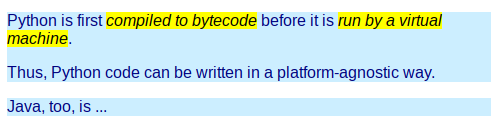
\includegraphics[width=\linewidth]{./gfx/22-html-divpspan}

\scriptsize
The following styles were used
\begin{itemize}
\item (default): 
	\begin{itemize}
	\scriptsize
	\item \texttt{font-family:sans-serif;}
    \item \texttt{font-style:normal;}
    \item \texttt{color:navy;}
	\end{itemize}
\item \texttt{language}: 
	\begin{itemize}
	\scriptsize
	\item \texttt{background-color:\#CCEEFF;}
	\end{itemize}
\item \texttt{highlight}: 
	\begin{itemize}
	\scriptsize
	\item \texttt{background-color:\#FFFF00;}
    \item \texttt{color:black;}
    \item \texttt{font-style:italic;}
	\end{itemize}
\end{itemize}
\end{defbox}

\end{tcbraster}
%
\end{frame}

% =========================================================================== %

\begin{frame}[fragile]{Hyperlinks and Bookmarks}
%
\begin{itemize}
\item Hyperlinks are coded with the \texttt{<a>} tag (see below)
	\begin{itemize}
	\item \enquote{Anchor} -- refers to an outdated use
	\item Syntax: \mintinline{html}{<a href="url">Link Text</a>}
	\end{itemize}
\pause
\item Bookmarks: \enquote{Links to scroll position}
	\begin{itemize}
	\item Define scroll position with \mintinline{html}{<a name="id" />} (outdated style)
	\item Or with \mintinline{html}{<tag id="id">...</tag>} (preferred today)
		\begin{itemize}
		\item \texttt{tag} is an arbitrary tag like \texttt{h1}, \texttt{p}, ...
		\end{itemize}
	\item In the link, use the pound symbol (\texttt{\#}) to refer to an anchor id:
		\begin{itemize}
		\item \mintinline{html}{<a href="#id">Link Text</a>}
		\end{itemize}
	\item May also be prepended to a regular URL
		\begin{itemize}
		\item \mintinline{html}{<a href="https://docs.python.org/3/library/functions.html#divmod">Link</a>}
		\item Note: In the HTTP context, anything behind \texttt{\#} is called \emph{the fragment} of the URL
		\end{itemize}
	\end{itemize}
\pause
\item Hyperlinks come with their own set of CSS properties
	\begin{itemize}
	\item Different styling depending on whether links are \emph{normal}, \emph{visited}, \emph{hovered over} or \emph{active}
	\item \url{https://www.w3schools.com/css/css_link.asp}
	\end{itemize}
\end{itemize}
%
\end{frame}

% =========================================================================== %

% tables
\begin{frame}{Tables}
%
\begin{itemize}
\item Parent tag: \texttt{table}
	\begin{itemize}
	\item Attributes \texttt{style} and \texttt{class} as usual
	\item CSS property \texttt{width}: Can be given in percent (\%) pixels (px), millimetres (mm), quarter millimetres (Q), inches (in) or sixth-inches (pc)
	\item CSS property \texttt{border}: Takes arguments like line width, dash-style, colour: \texttt{1px solid black}
	\item See \url{https://www.w3schools.com/html/html_table_borders.asp}
	\end{itemize}
\pause
\item For each row: add a tag-pair \texttt{<tr> ... </tr>}
\item For each cell within a row: add a tag-pair \texttt{<td> ... </td>}
\item Text in table only within \texttt{td} tags
\pause
\item Alternative for headings: tag-pair \texttt{<th> ... </th>}
\pause
\item \texttt{td} and \texttt{th} both support the \texttt{style} and \texttt{class} attributes
\item You can add styledefs for \texttt{td} and \texttt{tr} to one class
\end{itemize}
%
\end{frame}

% =========================================================================== %

\begin{frame}[fragile]
%
\begin{tcbraster}[raster columns=2,
                  raster equal height,
                  nobeforeafter,
                  raster column skip=0.1cm]
\begin{codebox}
\begin{minted}[fontsize=\scriptsize]{html}
<table style="width:150mm;
              border:3px solid;">
  <tr>
    <th style="border:1px solid;">a</th>
    <th style="border:1px solid;">b</th>
  </tr>
  <tr>
    <td>a</td>
    <td>b</td>
  </tr>
  <tr>
    <td>a</td>
    <td>b</td>
  </tr>
  <tr>
    <td>a</td>
    <td>b</td>
  </tr>
</table>
\end{minted}
\end{codebox}
%
\begin{defbox}[Output]
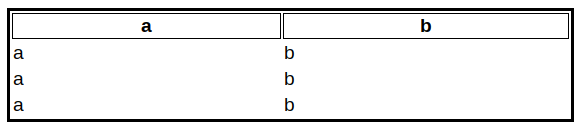
\includegraphics[width=\linewidth]{./gfx/22-html-table_1}

\scriptsize
See also online examples for the code behind this:
\vspace{-6pt}
\begin{center}
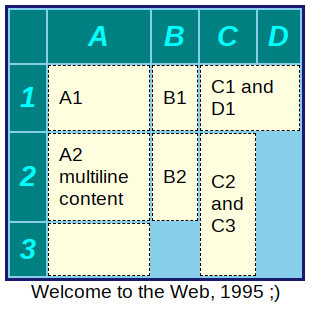
\includegraphics[width=.7\linewidth]{./gfx/22-html-table_2}
\end{center}
\end{defbox}

\end{tcbraster}
%
\end{frame}

% =========================================================================== %

\begin{frame}{Some Interactivity: Forms}
%
\begin{itemize}
\item Block \texttt{<form> ... </form>} enables some interactive elements
	\begin{itemize}
	\item Content: regular HTML tags plus \texttt{<input>}- and \texttt{<label>} tags
	\item \mintinline{html}{<input type="type" name="name">} adds an interactive element of type \texttt{type}:
		\vspace{-3pt}
		\begin{columns}[T]
		\column{.4\linewidth}
			\begin{itemize}
			\item \texttt{text} -- Text box
			\item \texttt{radio} -- Single Choice
			\item \texttt{checkbox} -- Check box
			\end{itemize}
		\column{.4\linewidth}
			\begin{itemize}
			\item \texttt{submit} -- Sends the form's content to the server
			\item \texttt{button} -- Triggers JavaScript code
			\end{itemize}
		\end{columns}

	\item \mintinline{html}{<label for="name>Text</label>} 
		\begin{itemize}
		\item Just adds \texttt{Text} to the website
		\item Clicking on \texttt{Text} also triggers the \texttt{input}
		\end{itemize}
	\end{itemize}
\pause
\item \texttt{form} has attributes \texttt{method}, \texttt{action} and \texttt{enctype}
	\begin{itemize}
	\item \texttt{method} should be a HTTP method (\zB \texttt{POST})
	\item \texttt{action} is an URL that tells the server what to do with these data
	\item \texttt{enctype} specifies how data is sent
		\begin{itemize}
		\item \texttt{application/x-www-form-urlencoded}: default; key:value-pairs, simple to parse
		\item \texttt{multipart/form-data}: for file uploads
		\end{itemize}
	\end{itemize}
\end{itemize}
%
\end{frame}

% =========================================================================== %

\begin{frame}[fragile]
%
\begin{codebox}
\begin{minted}[fontsize=\scriptsize]{html}
<form enctype="multipart/form-data" action="request_print" method="POST">
<table>
    <tr>
        <td><label for="file">File To Print:</label></td>
        <td><input type="file" name="file" /></td>
    </tr>
    <tr>
        <td><label for="PSF">Printer Settings File (PSF):</label></td>
        <td><input type="file" name="PSF" /></td>
    </tr>
    <tr style="height:30px; vertical-align:bottom;">
        <td colspan="2">Note: If no PSF is specified, default settings are used.</td>
    </tr>

    <tr>
        <td colspan="2"><input type="submit" value="Submit"></td>
    </tr>
</table>
</form>
\end{minted}
\end{codebox}
%
\end{frame}

% =========================================================================== %

\begin{frame}
%
\begin{hintbox}[That Belongs in a Muesum!]
Forms are hardly used by modern websites. JavaScript has all but replaced the technology because it provides much more versatility.

\vspace{3pt}
See \url{https://www.codemag.com/article/1701091} for some reasons why that is.

\vspace{3pt}
However, they \emph{are} still supported by common browsers, and won't die any time soon.
Without learning a new language, they provide an easy to use and straight forward means of providing an interface for a web-app.
And even if you are fluent in JavaScript (and at least one of its dozens of frameworks like NodeJS, Angular, ...), for some simple tasks like providing a contact form, using JS might be the equivalent of using an orbital laser cannon to boil a pot of water where forms are the ready made stove.
\end{hintbox}
%
\end{frame}

% =========================================================================== %

\begin{frame}{HTML Headers}
%
The tag block \texttt{<head> ... </head>} sets some useful properties
\pause
\begin{itemize}
\item \texttt{<title>...</title>} sets the string shown in the browser's title bar and on the tab
\pause
\item \texttt{<style> ... </style>} allows defining classes with CSS properties
	\begin{itemize}
	\item Syntax: \mintinline{css}{.classid {key:value; key:value; ...}}
	\item Without the \texttt{.} in front of \texttt{classid}, you define the default format for the regular tags!
	\end{itemize}
\pause
\item \texttt{<link>} adds references to other files
	\begin{itemize}
	\item What they mean is encoded in the \texttt{rel} attribute
	\item The referenced file is encoded in the \texttt{href} attribute
	\item E.\;g.: use a shared style sheet (CSS file):\\
		\mintinline{html}{<link rel="stylesheet" href="uri/to/file.css" />}
	\item E.\;g.: use an icon to display in the tabs bar:\\
		\mintinline{html}{<link rel="icon" href="uri/to/file.ico" />}
	\end{itemize}
\pause
\item \texttt{<meta />} tags contain information directed at search engines
	\begin{itemize}
	\item \mintinline{html}{<meta name="keywords" content="Coding, Python, IT" />}
	\end{itemize}
\pause
\item See \inPy{https://www.w3schools.com/html/html_head.asp} for more
\end{itemize}
%
\end{frame}

% =========================================================================== %

\begin{frame}[fragile]{Python Package \texttt{html.parser}}
%
\begin{itemize}
\item Class \texttt{HTMLParser} can be used as a base class for interpreting HTML-like files
\item User should override three methods:
	\begin{itemize}
	\item \inPy{def handle_starttag(self, tag, attrs)} -- called when an open tag is encountered
	\item \inPy{def handle_endtag(self, tag)} -- called when an tag is closed
	\item \inPy{def handle_data(self, data)} -- called when contained text is encountered
	\end{itemize}
\pause
\item Method \texttt{feed(html\_document)} sends a string into the parser
\pause
\item[\Thus] The \texttt{starttag} and \texttt{endtag} methods set instance attributes
\item[\Thus] The \texttt{data} method triggers rendering
\pause
\item See \url{https://docs.python.org/3/library/html.parser.html} for details
\end{itemize}
%
\end{frame}

% =========================================================================== %

\begin{frame}[fragile]
%
\begin{tcbraster}[raster columns=2,
                  raster equal height,
                  nobeforeafter,
                  raster column skip=0.1cm]
\begin{codebox}[Example]
\begin{minted}[linenos, fontsize=\scriptsize]{python3}
from html.parser import HTMLParser

class MyHTMLParser(HTMLParser):
    def handle_starttag(self, tag, attr):
        print(f"Opening tag: {tag:5}",
              "with attributes", attr)
    def handle_endtag(self, tag):
        print(f"Closing tag : {tag:5}")
    def handle_data(self, data):
        print("Parsing data:", 
              data.strip())

parser = MyHTMLParser()
parser.feed("""<html>
<head><title>Test</title></head>
<body>
<h1 style="color:navy">Parse me!</h1>
</body>
</html>""")
\end{minted}
\end{codebox}
%
\begin{cmdbox}[Output]
\begin{minted}[fontsize=\scriptsize]{text}
Opening tag : html  with attributes []
Parsing data:
Opening tag : head  with attributes []
Opening tag : title with attributes []
Parsing data: Test
Closing tag : title
Closing tag : head 
Parsing data:
Opening tag : body  with attributes []
Parsing data:
Opening tag : h1    with attributes 
             [('style', 'color:navy')]
Parsing data: Parse me!
Closing tag : h1   
Parsing data:
Closing tag : body 
Parsing data:
Closing tag : html
\end{minted}
\end{cmdbox}
\end{tcbraster}
%
\end{frame}

% =========================================================================== %

\begin{frame}{Fantastic XMLs and Where to Find Them}
%
\begin{itemize}
\item XML-Like documents can do more than convey rendering information
\item Store any text-based tree structure
	\begin{itemize}
	\item Integrated distinction between information (text) and meta-data (attributes)
	\end{itemize}
\item[\Thus] Very common format for program settings
\pause
\item Example 1: PyCharm (or any JetBrains IDE)
	\begin{itemize}
	\item Go to (hidden) folder \texttt{.idea} in any project directory
	\item Find various .xml files and an .iml file therein!\\
	 	The .iml only has a different extension but also follows xml syntax
	\end{itemize}
\pause
\item Example 2: Office Suite Files
	\begin{itemize}
	\item Take any file produced by Microsoft Office or LibreOffice (\zB a .docx file or a .odf file)
	\item Rename it to .zip
	\item Find a lot of XML files describing your document!
	\item See \url{https://en.wikipedia.org/wiki/OpenDocument_technical_specification} for more details
	\end{itemize}
\end{itemize}
%
\end{frame}

% =========================================================================== %

\begin{frame}{Python Package \texttt{xml.etree.ElementTree}}
%
\begin{itemize}
\item \texttt{ElementTree} is an efficient xml Parser for Python
\item Reading and writing capabilities
\item Convention: \inPy{import xml.etree.ElementTree as ET}
\pause
\item Class \texttt{ET.ElementTree} models the XML document
	\begin{itemize}
	\item Obtained from \texttt{ET.parse(filename\_as\_string}
	\item Or from \texttt{ET.fromstring(xml\_code\_as\_string)}
	\end{itemize}
\pause
\item \texttt{ElementTree} is a collection of \texttt{Element}s
	\begin{itemize}
	\item \texttt{Element} has attributes \texttt{tag}, \texttt{text} (both \inPy{str}ing) and \texttt{attrib} (\inPy{dict})
	\end{itemize}
\pause
\item \texttt{Element} is \emph{iterable}
	\begin{itemize}
	\item Iteration runs over all tags directly under the \texttt{Element}
	\end{itemize}
\pause
\item \texttt{ElementTree} has method \texttt{iter} (not \inPy{__iter__})
	\begin{itemize}
	\item Still returns an iterator
	\item Iteration runs over all tags in the tree, in order of appearence
	\item No Information about ownership in this way
	\end{itemize}
\end{itemize}
%
\end{frame}

% =========================================================================== %

\begin{frame}[fragile]
%
\begin{tcbraster}[raster columns=2,
                  raster equal height,
                  nobeforeafter,
                  raster column skip=0.1cm]
\begin{codebox}[Example Document]
\begin{minted}[linenos, fontsize=\tiny]{xml}
<?xml version="1.0"?>
<data>
    <country name="Liechtenstein">
        <rank>1</rank>
        <year>2008</year>
        <gdppc>141100</gdppc>
        <neighbor name="Austria" direction="E"/>
        <neighbor name="Switzerland" direction="W"/>
    </country>
    <country name="Singapore">
        <rank>4</rank>
        <year>2011</year>
        <gdppc>59900</gdppc>
        <neighbor name="Malaysia" direction="N"/>
    </country>
    <country name="Panama">
        <rank>68</rank>
        <year>2011</year>
        <gdppc>13600</gdppc>
        <neighbor name="Costa Rica" direction="W"/>
        <neighbor name="Colombia" direction="E"/>
    </country>
</data>
\end{minted}
\end{codebox}
%
\begin{defbox}[Vizualization]
	\begin{minipage}{.35\linewidth}
	% [trim={left bottom right top},clip]
	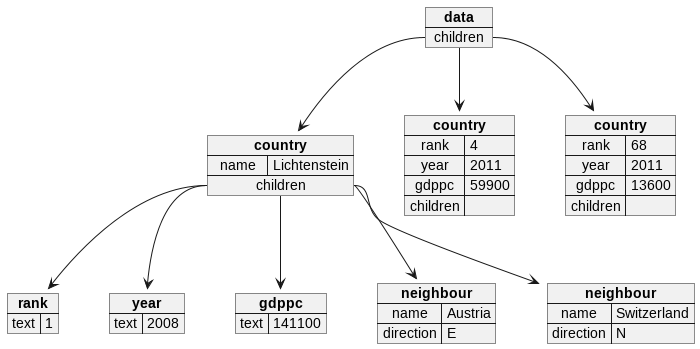
\includegraphics[width=\linewidth, trim={2cm 2cm 12cm 2cm}, clip]{./gfx/22-xml-countries}
	\end{minipage}
	%
	\begin{minipage}{.60\linewidth}
	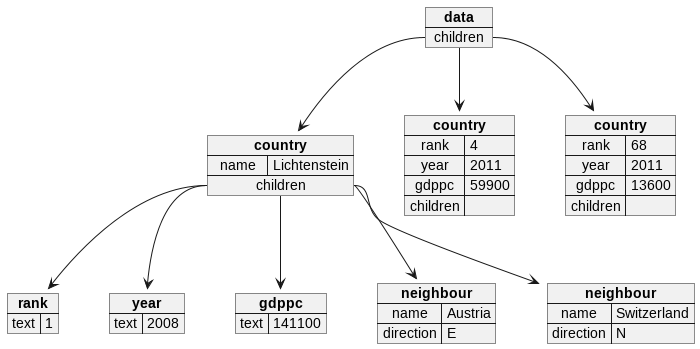
\includegraphics[width=\linewidth, trim={2cm 18.5cm 12cm 2cm}, clip]{./gfx/22-xml-countries}
	\end{minipage}
\end{defbox}
\end{tcbraster}
%
\end{frame}

% =========================================================================== %

\begin{frame}[fragile]
%
\vspace{-0.7cm}
\begin{columns}
\column{.7\linewidth}
\begin{codebox}[ElementTree Example]
\begin{minted}[linenos, fontsize=\scriptsize]{python3}
import xml.etree.ElementTree as ET
tree = ET.parse('country_data.xml')    # type ElementTree
root = tree.getroot()                  # type Element

print(root.tag)                        # 'data'
print(root.attrib)                     # {}

for child in root:                     # all direct children
    print(child.tag, child.attrib)
# country {'name': 'Liechtenstein'}
# country {'name': 'Singapore'}
# country {'name': 'Panama'}

for neighbor in root.iter('neighbor'): # any depth, filtered
    print(neighbor.attrib)
# {'name': 'Austria', 'direction': 'E'}
# {'name': 'Switzerland', 'direction': 'W'}
# {'name': 'Malaysia', 'direction': 'N'}
# {'name': 'Costa Rica', 'direction': 'W'}
# {'name': 'Colombia', 'direction': 'E'}
\end{minted}
\end{codebox}
%
\column{.16\linewidth}
\vspace{1cm}
% [trim={left bottom right top},clip]
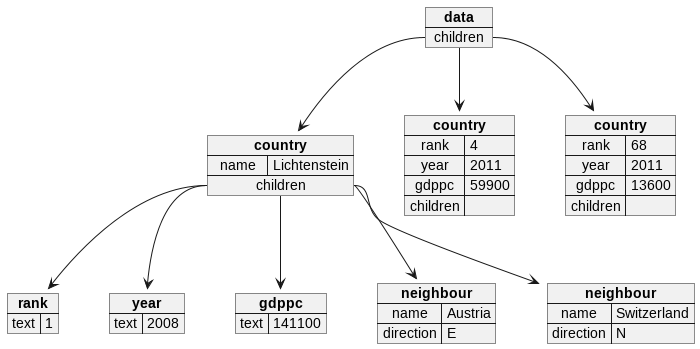
\includegraphics[width=\linewidth, trim={2cm 2cm 12cm 2cm}, clip]{./gfx/22-xml-countries}
\end{columns}
%
\end{frame}

% =========================================================================== %

\begin{frame}[fragile]
%
\vspace{-0.7cm}
\begin{columns}
\column{.7\linewidth}
\begin{codebox}[... continued]
\begin{minted}[linenos, firstnumber=last, fontsize=\scriptsize]{python3}
print(root[0].attrib)                # {'name': 'Singapore'}
print(root[0][1].text)               # 2008

for rank in root.iter('rank'):
    new_rank = int(rank.text) + 1
    rank.text = str(new_rank)
    rank.set('updated', 'yes')       # adds attribute

tree.write('output.xml')

# ---------------------------------------
# building an ElementTree from scratch:

a = ET.Element('a')
b = ET.SubElement(a, 'b')
c = ET.SubElement(a, 'c')
d = ET.SubElement(c, 'd')
print(ET.dump(a))
# <a><b /><c><d /></c></a>
\end{minted}
\end{codebox}
%
\column{.16\linewidth}
\vspace{1cm}
% [trim={left bottom right top},clip]
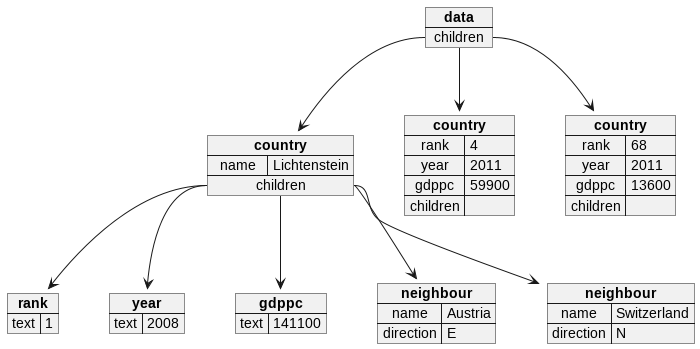
\includegraphics[width=\linewidth, trim={2cm 2cm 12cm 2cm}, clip]{./gfx/22-xml-countries}
\end{columns}
%
\end{frame}

% =========================================================================== %

\begin{frame}{Links}
%
\begin{itemize}
\item Python Docs
	\begin{itemize}
	\item \url{https://docs.python.org/3/library/xml.etree.elementtree.html}
	\item \url{https://docs.python.org/3/library/html.parser.html}
	\item \url{https://docs.python.org/3/library/html.entities.html}
	\end{itemize}
\item W3Schools
	\begin{itemize}
	\item \url{https://www.w3schools.com/html/default.asp}
	\item \url{https://www.w3schools.com/css/default.asp}
	\item \url{https://www.w3schools.com/xml/default.asp}
	\end{itemize}
\item Mozilla Dev Network
	\begin{itemize}
	\item \url{https://developer.mozilla.org/en-US/docs/Web/HTML}
	\item \url{https://developer.mozilla.org/en-US/docs/Web/CSS}
	\end{itemize}
\item HTML Entities
	\begin{itemize}
	\item \url{https://symbl.cc/en/html-entities/}
	\end{itemize}
\end{itemize}
%
\end{frame}

% =========================================================================== %
\end{document}

% MAREI!!
% whom do I give credit? Where?